\documentclass[UKenglish]{article}  %% ... or USenglish or norsk or nynorsk
\usepackage[utf8]{inputenc}           %% ... or latin1 or applemac
\usepackage[T1]{fontenc,url}
\urlstyle{sf}
\usepackage{tikz,babel,textcomp,csquotes,pgf-umlsd,varioref,graphicx}
\usetikzlibrary{arrows, shadows}
\title{Project 1}        %% ... or whatever
         %% ... if any
\author{Aulon Mujaj, Henning Lund-Hanssen, Espen Jones}                      %% ... or whoever 

\begin{document}
\maketitle{}

\section{Requirement 1 - Brief analysis}

\subsection{Brief description}
This program is a simulation of the popular game Minesweeper. In this version of
Minesweeper, the player is presented with a map of coordinates with
questionmarks. Under each questionmark, there is either a number representing
how many mines that are in the vicinity of this particular point on the map, or,
a mine. The player is prompted for a set of coordinates, which should correlate
to a questionmark on the map that the player does not think has a mine beneath
it. The game goes on for as long as the player does not hit a questionmark with
a mine beneath. The game ends when the player has identified all of the
questionmarks without a mine, or if the player hits a questionmark with a mine.
\subsection{Analysis}
\subsubsection{Defects}
This program consists of three files.

\begin{itemize}
    \item Minesweeper.java - The main class of this program. Calls on the two other parts, MineField and Ranking.
    \item MineField.java - Represents the map of the minefield
    \item Ranking.java - Handles the highscores of the players playing this game
\end{itemize}
\subsubsection{Minesweeper.java}
This main class on the program has the responsibility for the control flow of the program. When should the minefield be
called to make a judgement about whether the game is still going or ended? When should the ranking be upon to calculate
the score of the player and show the highscore? It taks input from the terminal and compares it to certain keywords. If
the input from the player does not match the input criteria, the game just prompts for new input.

The testable parts in this class consist of handling the input from the user and that the right action is taken
accordingly. For example, if the user gives "top" as input to the program, the ranking class should be called to show
the ranking of the players. And if restart is called, you would expect the program to restart your session.
\subsubsection{MineField.java}

\subsubsection{Ranking.java}
\subsection{Non-functional tests}
In our opinion, the Minesweeper program does not display the need for non-functional tests. It is Java, so it to a high
degree platform independent. It is Java, so it to a high degree platform independent. CONTINUE HERE HENNING

\subsection{Test cases}

\section{Requirement 2 - In-depth metrics}

\subsection{Metrics at project level}
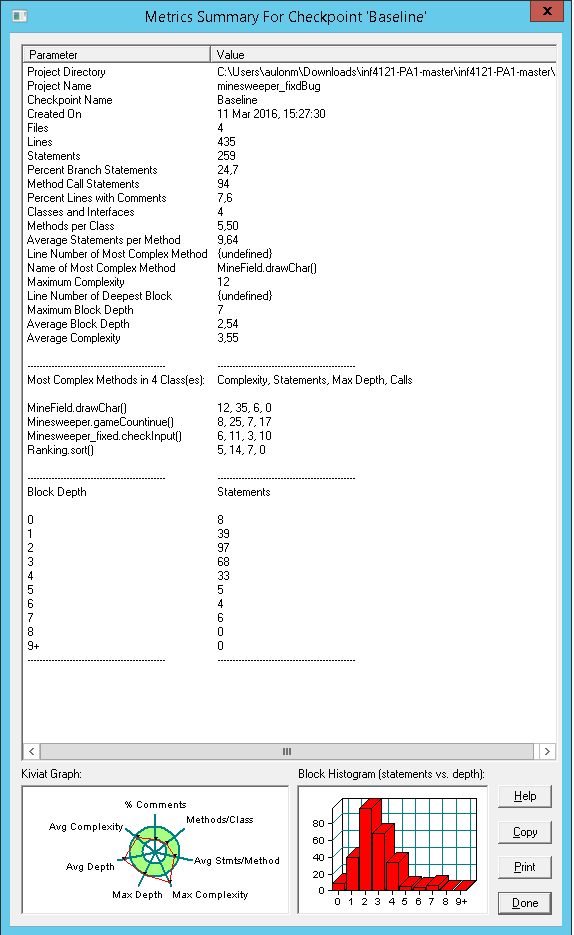
\includegraphics[height=8cm]{metric_summary}
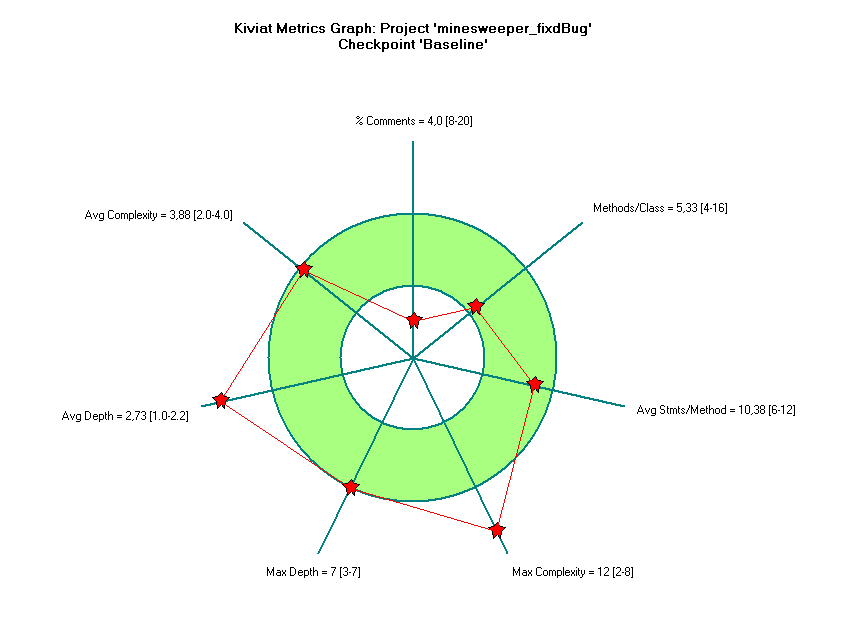
\includegraphics[height=8cm]{kiviat_diagram_baseline}
\begin{itemize}
\item What metrics do you spot for the whole project in the window Metrics Summary for Checkpoint? Write a brief description of the metrics. Try to explain their values (below what is expected, as expected or above the expected level). What metrics do you think need to change?\\
\item Which is the biggest file you have in your project by the number of lines of code? \\
MineField.java
\item Which is the file with most branches in your project?\\
\item Which is the file with most complex code? What metric did you choose to answer to this question?\\
Minesweeper.java
\end{itemize}

Write a little about each metric, maybe we'll only write about the 6 different metrics from the kiviat diagram, instead of each metric from the metric summary image?

If we choose to go only for the metrics from the kiviat diagram, then we'll only need to write about:\\
Avg complexity, avg depth, max depth, \% comments, methods/class, avg stats/method, max complexity\\

Statements:
Branch statements:
Method call statements:
Percent lines with comments:
Classes and Interfaces
Methods per class:
Average Statements per Method:
Name of Most complex methods
Maximum Complexity
Maximum Block Depth
Average Block Depth
Average Complexity
Most complext methods (complexity, statements, max depth, calls)
How many statements on each block depth



\subsection{Metrics at file level}
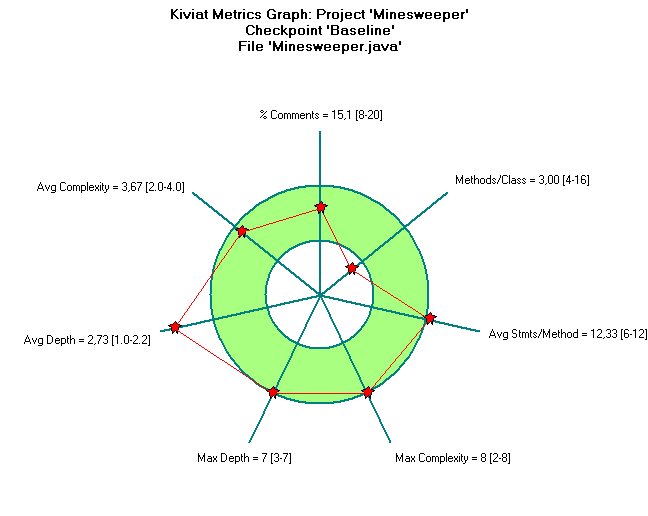
\includegraphics[height=8cm]{kiviat_diagram_minesweeper}
\begin{itemize}
\item How do you interpret the metrics applied on your file? How are they different the metrics you optained on the whole project, compared with the metrics ont his file?\\
\item Would you refactor (re-write) any of the methods you have in this file?
\end{itemize}
\section{Requirement 3 - Code improvement}

\subsection{Identification of metrics}

\subsection{Results from changes}

\subsection{Final remarks}

\end{document}
